\section{Đánh giá mô hình đã chọn trên tập kiểm tra}
\label{sec:6_5}
Mô hình được đánh giá là \texttt{mlp\_32\_reg}, MLP một lớp ẩn 32 nút với $\alpha=0{,}01$, đã được chọn bằng F1 CV ở bước 5. Đầu vào dùng median, mode, one-hot và StandardScaler trên sáu biến số, không PCA. Mô hình đã fit trên 26.049 mẫu train; không fit thêm bằng validation hoặc test. Ngưỡng xác suất lớp \texttt{>50K} giữ nguyên ở 0,5.

Trước khi đánh giá, pipeline và thông tin lựa chọn được sao lưu cố định ở \texttt{artifacts/final/}. SHA-256 và trạng thái fitted được kiểm tra trước/sau dự đoán. Module đánh giá không gọi fit, không tìm ngưỡng tối ưu và không so sánh thêm các mô hình trên test để đổi lựa chọn. Lần chạy lại với cùng snapshot và dữ liệu đọc kết quả đã xác minh thay vì mở một thí nghiệm lựa chọn mới.

Tập test là toàn bộ 16.281 dòng \texttt{adult.test} gốc sau khi chuẩn hóa định dạng như bước 1, gồm 12.435 mẫu \texttt{<=50K} và 3.846 mẫu \texttt{>50K}. Mã hóa nhãn không thay số dòng hay thứ tự. Các mục dưới đây trình bày kết quả test; không gộp chúng với điểm CV/validation.

\subsection{Các chỉ số đánh giá}
\label{subsec:6_5_1}
Các chỉ số được tính từ nhãn test và dự đoán cố định; lớp dương là \texttt{>50K}. Accuracy đạt 85,56\%, nhưng recall lớp dương chỉ đạt 62,48\%. Vì vậy, tỷ lệ dự đoán đúng tổng thể không đủ để mô tả khả năng nhận diện nhóm thu nhập cao.

\begin{table}[htbp]
\centering\small
\caption{Các chỉ số trên toàn bộ tập test với ngưỡng đã khóa}\label{tab:test-metrics}
\begin{tabular}{lr}
\toprule
Chỉ số & Giá trị \\
\midrule
Accuracy & 0,8556 \\
Precision lớp >50K & 0,7258 \\
Recall lớp >50K & 0,6248 \\
F1 lớp >50K & 0,6715 \\
Macro-F1 & 0,7895 \\
ROC-AUC & 0,9093 \\
Average precision (AP) & 0,7741 \\
Specificity & 0,9270 \\
False positive rate (FPR) & 0,0730 \\
False negative rate (FNR) & 0,3752 \\
Balanced accuracy & 0,7759 \\
\bottomrule
\end{tabular}
\end{table}
\begin{table}[htbp]
\centering\small
\caption{Kết quả test theo từng lớp}\label{tab:test-per-class}
\begin{tabular}{lrrrr}
\toprule
Lớp & Precision & Recall & F1 & Số mẫu \\
\midrule
\texttt{<=50K} & 0,8887 & 0,9270 & 0,9075 & 12.435 \\
\texttt{>50K} & 0,7258 & 0,6248 & 0,6715 & 3.846 \\
\bottomrule
\end{tabular}
\end{table}
Precision 0,7258 và recall 0,6248 cho thấy tại ngưỡng 0,5 mô hình vẫn bỏ sót một phần mẫu dương. Specificity bằng 0,9270 mô tả tỷ lệ nhận diện đúng lớp âm; FPR bằng 0,0730 là tỷ lệ mẫu âm bị dự đoán thành dương. Macro-F1 và balanced accuracy cho mỗi lớp vai trò cân bằng hơn so với accuracy tổng thể.

ROC-AUC và AP sử dụng score lớp dương để đánh giá thứ hạng qua nhiều ngưỡng. AP là tổng có trọng số theo bước tăng recall, không được đồng nhất với diện tích PR tính bằng quy tắc hình thang~\cite{sklearn-ap}. Không dùng các đường cong test để chọn lại ngưỡng.

\subsection{Ma trận nhầm lẫn và đường cong đánh giá}
\label{subsec:6_5_2}
Hàng của ma trận là nhãn thật, cột là nhãn dự đoán; thứ tự lớp là \texttt{<=50K}, \texttt{>50K}. Với quy ước này, hàng thứ nhất lần lượt là TN, FP; hàng thứ hai lần lượt là FN, TP~\cite{sklearn-cm}. Kết quả gồm TN=11.527, FP=908, FN=1.443 và TP=2.403.

\begin{figure}[htbp]
\centering
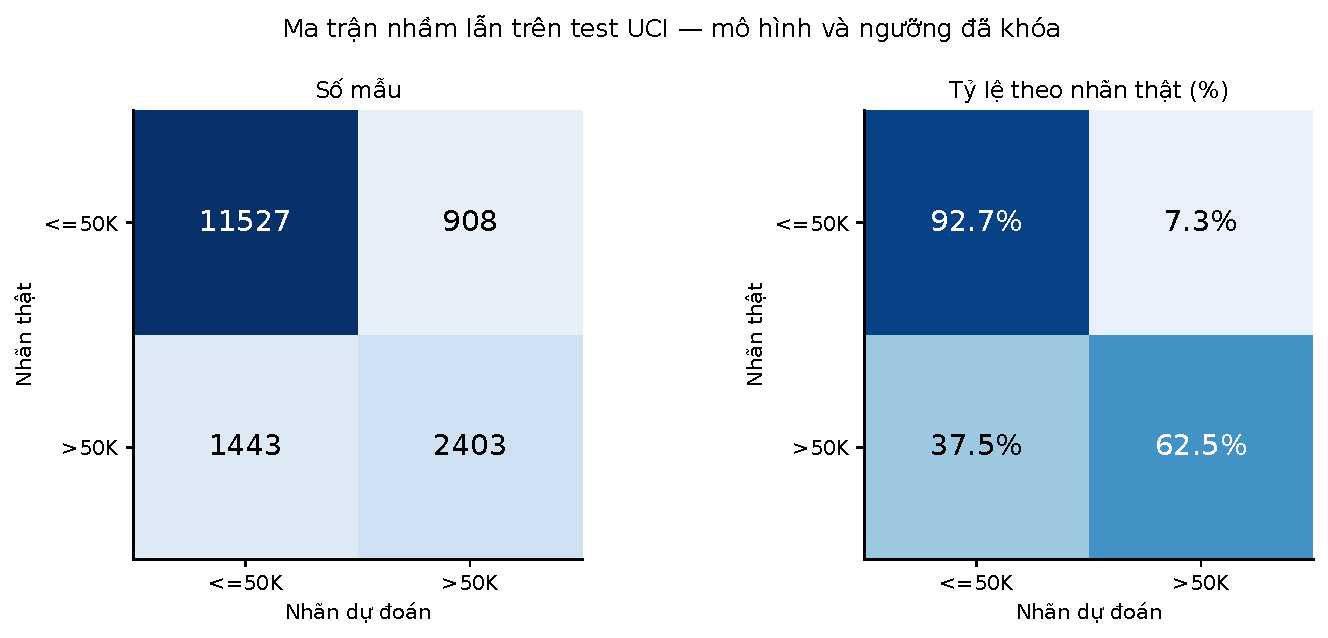
\includegraphics[width=.98\textwidth]{Images/chapter_6/6_5/6_5_2/test_confusion_matrix.pdf}
\caption{Ma trận nhầm lẫn: số mẫu và tỷ lệ chuẩn hóa theo hàng}\label{fig:test-cm}
\end{figure}

\begin{figure}[htbp]
\centering
\begin{minipage}{.49\textwidth}\centering
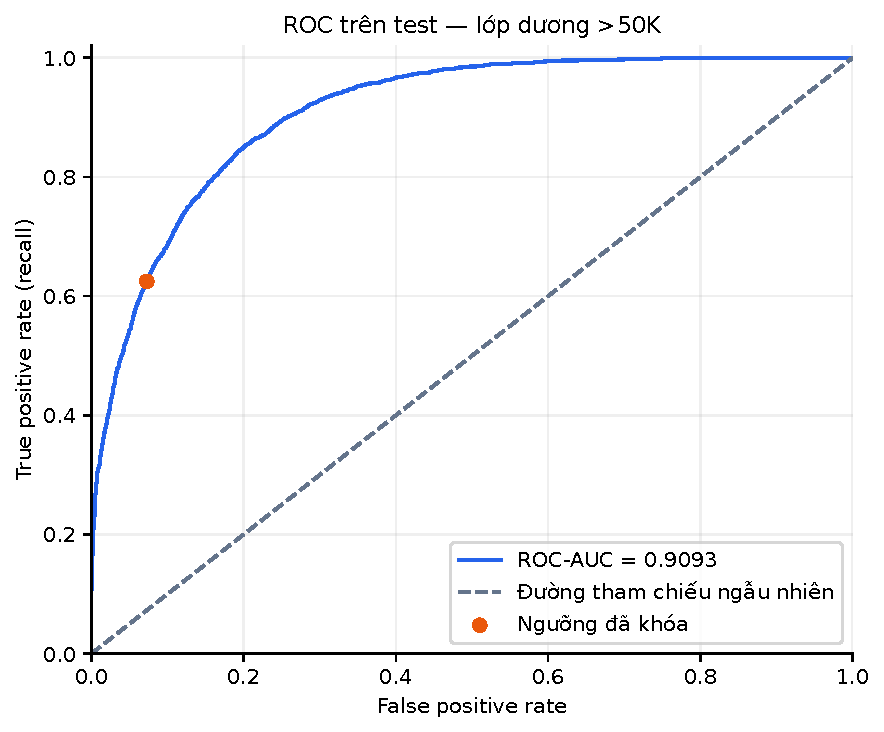
\includegraphics[width=\linewidth]{Images/chapter_6/6_5/6_5_2/test_roc.pdf}
\end{minipage}\hfill
\begin{minipage}{.49\textwidth}\centering
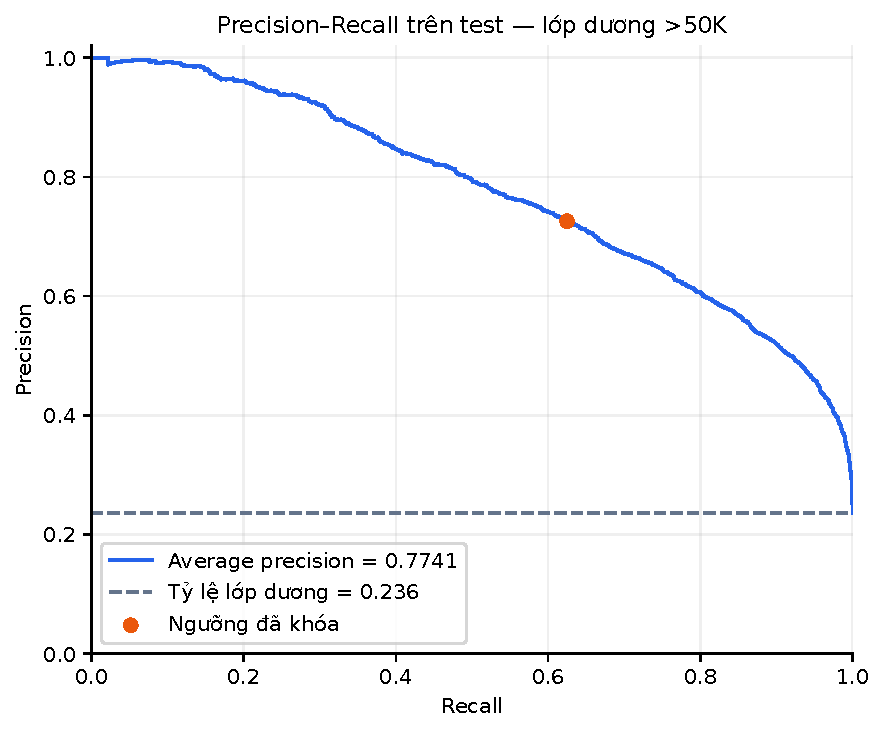
\includegraphics[width=\linewidth]{Images/chapter_6/6_5/6_5_2/test_precision_recall.pdf}
\end{minipage}
\caption{Đường ROC và Precision--Recall trên test; chấm đánh dấu là ngưỡng 0,5 đã khóa}\label{fig:test-curves}
\end{figure}

Mẫu bỏ sót FN chiếm 37,52\% số mẫu dương, trong khi FP chiếm 7,30\% số mẫu âm. Tỷ lệ lớp dương trên test là 23,62\%, được vẽ làm đường tham chiếu trên biểu đồ PR. Các đường cong mô tả sự đánh đổi nếu thay ngưỡng; bài làm giữ nguyên điểm vận hành đã chọn trước khi xem test.

